\section{Park Generation}

Once the plot generation is finished, the park generation starts filling some of the plots with parks.
The parks are generated through two steps, the first step is to generate a natural-looking path, and the second step is to fill the park with objects such as trees, bushes, and rocks.

The algorithm for generating paths works by first generating a random point on one of the edges of the plot and then scattering points randomly inside the plot with a minimum distance from one another.
The points are then sorted by distance, ensuring that the path always traverses to the closest possible point.
Afterward, once all points are found, the algorithm either creates a path that loops back to the starting point, or a path towards another random point on the edge of the plot (see Figure~\ref{fig:parks}).
Finally, exits/entries are added to the park by creating more paths to the edges of the plot.

The algorithm for object placement runs after paths are created to ensure that objects do not intersect with the generated path.
The first step of this algorithm is to assign each object type with an object radius, indicating the distance at which other objects are allowed to be created.
Afterward, a probability of being generated is assigned to each object type.
The algorithm then runs several times, and each time an object-type is picked, a model of that object-type is randomly chosen, scaled, and rotated before being generated and placed somewhere in the park.

\begin{figure}[H]
  \centering
  \begin{subfigure}[b]{0.45\textwidth}
    \frame{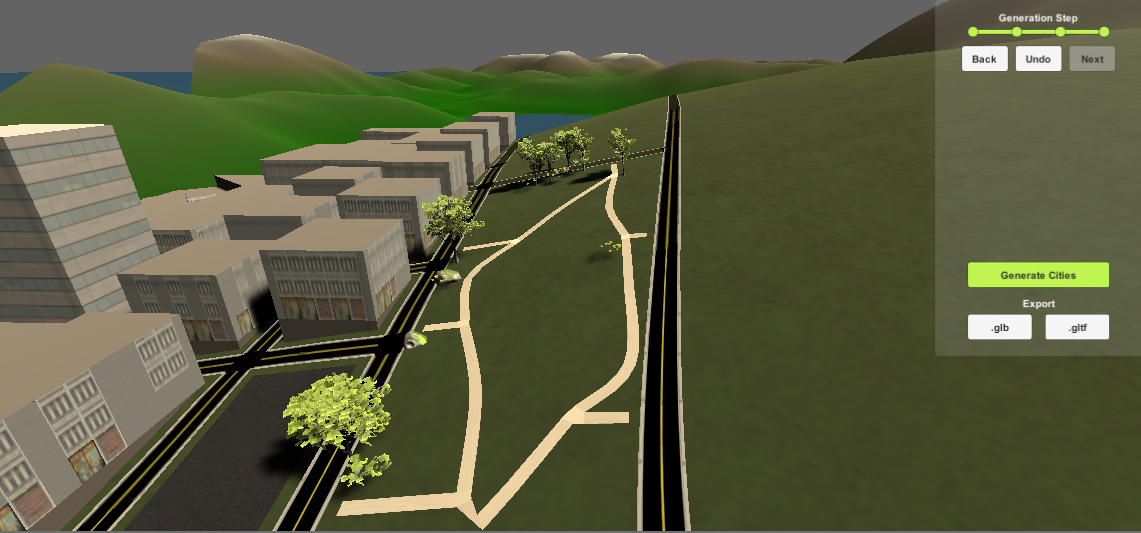
\includegraphics[width=\textwidth]{figure/resultpark3}}
    \caption{Park with looping path.}
  \end{subfigure}
  \quad
  \begin{subfigure}[b]{0.45\textwidth}
    \frame{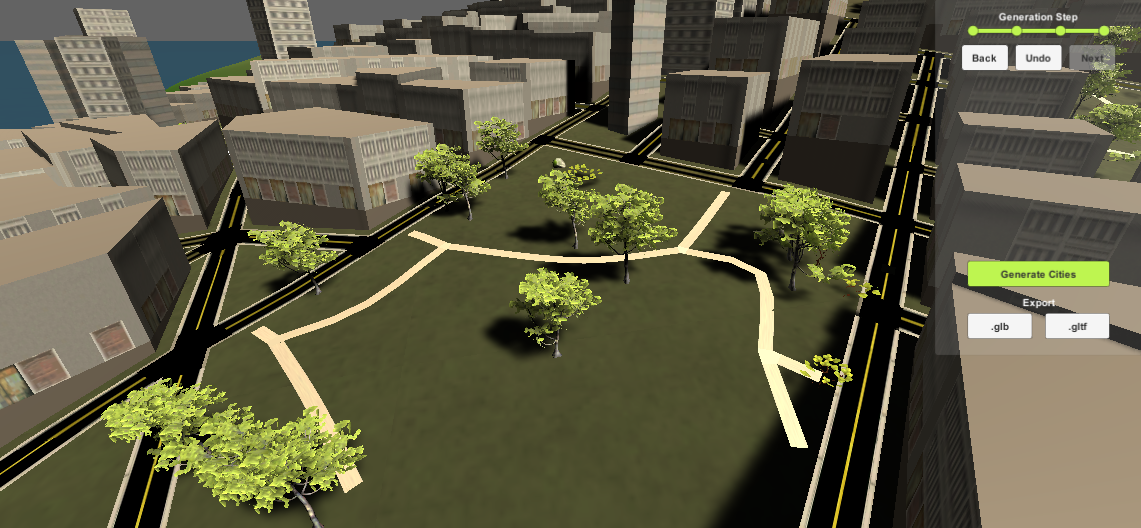
\includegraphics[width=\textwidth]{figure/resultpark2}}
    \caption{Park with path that does not loop.}
  \end{subfigure}
  \caption{Two example of different generated parks. One with a path that loops back, and one that creates a path to another edge of the plot.}
  \label{fig:parks}
\end{figure}

It is worth noting that even though the paths always end up looping, or connecting to a random edge, their shapes still vary a lot, leading to quite interesting results (see Figure~\ref{fig:park_ex2}).
The fact that object placement takes the path into account also makes the park layout appear less random and more relative to its environment.
This provides a more consistent feeling to the different parks.

\begin{figure}[H]
  \centering
  \begin{subfigure}[b]{0.45\textwidth}
    \frame{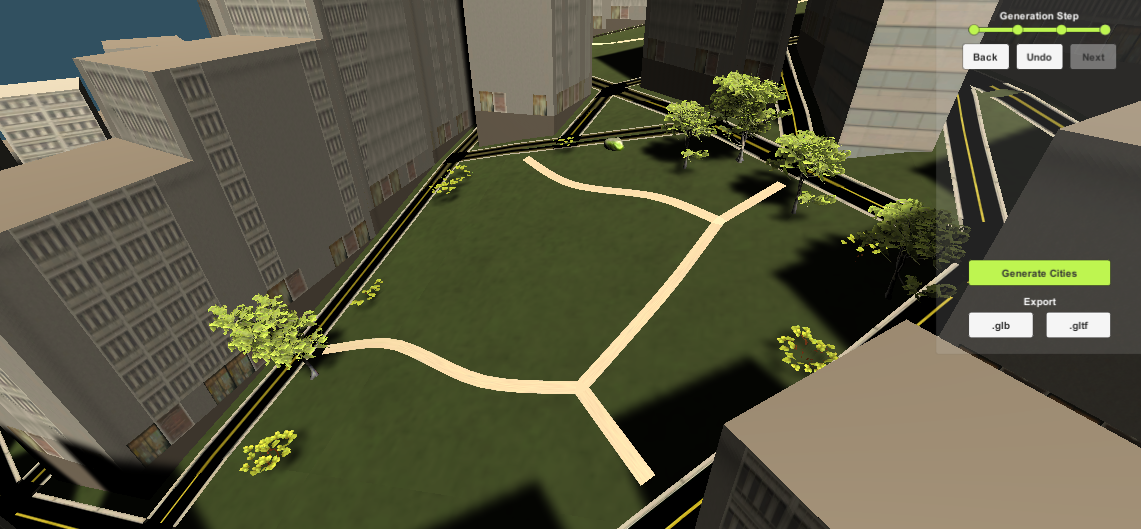
\includegraphics[width=\textwidth]{figure/resultpark1}}
  \end{subfigure}
  \quad
  \begin{subfigure}[b]{0.45\textwidth}
    \frame{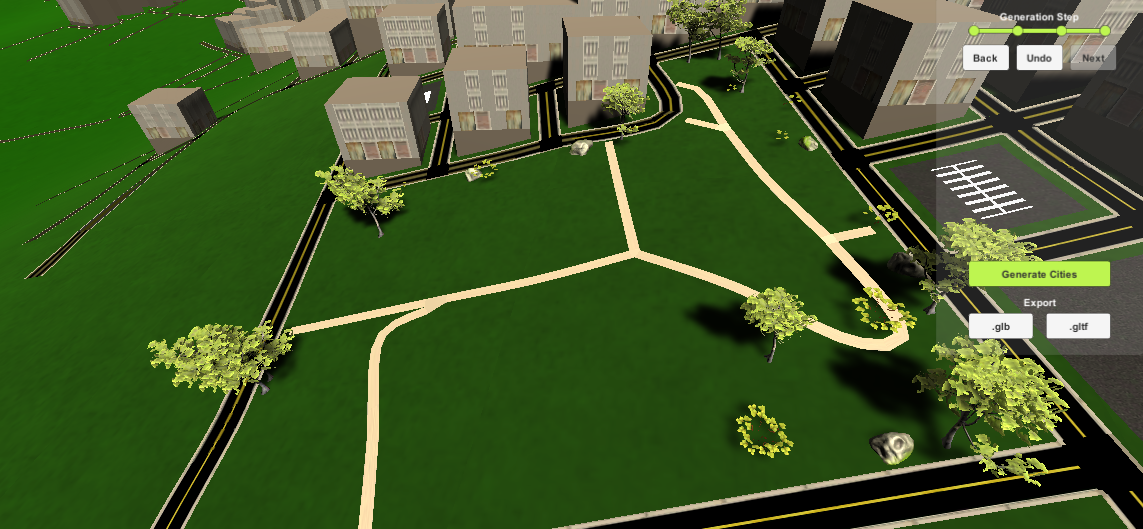
\includegraphics[width=\textwidth]{figure/resultpark4}}
  \end{subfigure}
  \caption{Two additional examples, showcasing different results.}
  \label{fig:park_ex2}
\end{figure}
